\section{Probabilistic Completeness of Global Planning}
\label{sec:analysis}



Proving probablistic completeness in $\pspace$ is challenging due to the multi-modal nature of the problem. Specifically, as the virtual elastic band moves in and out of contact the dimensionality of the manifold that the system is operating in can change. In addition, the virtual elastic band forward propagation function (Alg.~\ref{alg:band_propogation}) can allow the band to ``snap tight'' as the grippers move past the edge of an obstacle, changing the number of points in the band representation as it does so. By leveraging the assumptions from Sec.~\ref{sec:rpath_assumptions}, we are able to bypass most of these challenges by focusing on the portion of $\pspace$ that can be analyzed; i.e. $\robotCspace$.



This section proves the probabilistic completeness of the planning approach in two major steps.  First, it will show that the approach for selecting the nearest node in the tree for expansion is equivalent to performing a nearest-neighbor query in the full space.  Second, it proves that our algorithm will eventually return a path that is $\deltar$-similar to an optimal $\delta$-robust solution to the planning problem with probability 1 (if it exists), or it will terminate early having found an alternate path to the goal region. Recall that we do not require an optimal path, only a feasible one.


\begin{figure}
    \centering
    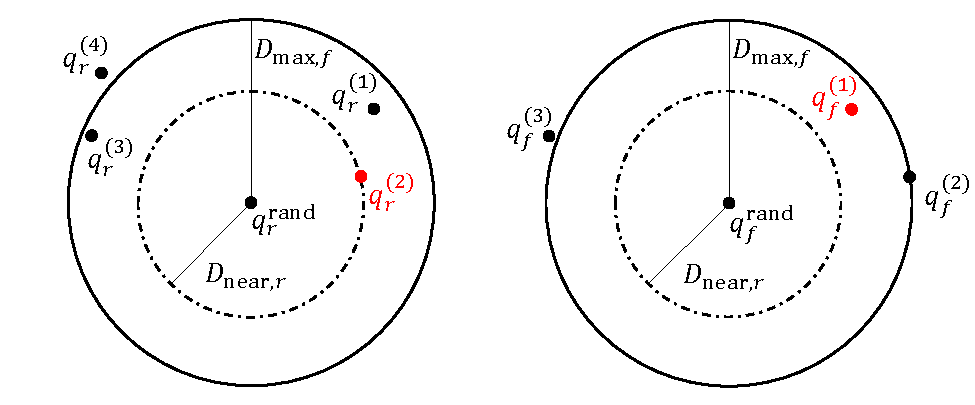
\includegraphics[width=0.7\columnwidth]{nearest_neighbour}
    \caption{Left: $\robotconfig^{(2)}$ is the nearest node to the $\pstaterand$ in robot space, but it my be as far as $\Dmaxf$ away in the full configuration space. By considering all nodes within $\Dmaxf$ in robot space, we ensure that any node (such as $\pstate^{(1)}$) that is closer to $\pstaterand$ than $\pstate^{(2)}$ is selected as part of $\Pstatenear$, while nodes such as $\pstate^{(4)}$ are excluded in order to avoid the expense of calculating the full configuration space distance. Right: we then measure the distance in the full configuration space to all nodes that could possibly be the nearest to $\pstaterand$, returning $\pstate^{(1)}$ as the nearest node in the tree.}
    \label{fig:nearest}
\end{figure}






\subsection{Assumptions and Definitions:}
\label{sec:rpath_assumptions}
Our problem allows for the virtual elastic band to be in contact with the surface of an obstacle, both during execution and as part of the goal set; this means that common assumptions regarding the expansiveness (\cite{Hsu1999}) of the planning problem may not hold. Instead of relying on expansiveness, we will define a series of alternate definitions and assumptions which are sufficient to ensure the completeness of our method.


First, in line with prior work, we will be assuming properties of the problem instance in regards to robustness.  In particular, we will be assuming the existence of a solution to a given query $\refpathf : [0, 1] \rightarrow \pspacevalid$ which has several robustness properties.  This solution is called a reference path.


To begin describing the properties of the reference path, we assume $\refpathf$ has robustness properties in the robot configuration space.  That is, the corresponding path in robot configuration space $\refpathr$ has strong $\deltar$-clearance under distance metric $d_\robotconfig(\cdot,\cdot)$ for some $\deltar > 0$.

\begin{definition}[Strong $\delta$-clearance]
    A path $\configpath : [0, 1] \rightarrow \pspacevalid$ has strong $\delta$-clearance under distance metric $d(\cdot,\cdot)$ if $\forall s \in [0, 1],\; d(\configpath(s), \pspaceinv) \geq \delta$, for $\delta > 0$.
\end{definition}

Given our assumption about the $\deltar$-clearance of the reference path in robot space, there exists a set $\setofpathsr$ of $\deltar$-similar paths to the reference path which are also collision-free.


\begin{definition}[$\delta$-similar path]
    Two paths $\configpath_a$ and $\configpath_b$ are $\delta$-similar if the Fr\'echet distance between the paths is less than or equal to $\delta$.
\end{definition}

Informally the Fr\'echet distance is described as follows~\cite{Alt1995Frechet}: Suppose a man is walking a dog. The man is walking on one curve while the dog on another curve. Both walk at any speed but are not allowed to move backwards. The Fr\'echet distance of the two curves is then the minimum length of leash necessary to connect the man and the dog.


Given the relationship between robot-space and full-space paths, we can define a full-space equivalent to $\setofpathsr$ as
\begin{equation}
    \setofpathsf = \{ \pspacepath \mid \rspacepath \in \setofpathsr \textrm{ and } \pspacepath = \textrm{FullSpace}(\rspacepath, \pstateinit) \} \enspace .
\end{equation}

Given these assumptions and definitions, we are ready to define an \textit{acceptable $\delta$-robust path}:
\begin{definition}[Acceptable $\delta$-Robust Path]
\label{def:robust}
A path $\refpathf$ is acceptable $\delta$-robust if the following hold:
\begin{enumerate}
    \item The robot-space reference path $\refpathr$ has strong $\deltar$-clearance for some $\deltar > 0$;
    \item The final state for every path $\pspacepath \in \setofpathsf$ is in $\Pspacegoal$. 
\end{enumerate}
\end{definition}
\noindent We assume there exists a reference path which satisfies this property and answers our given planning query:

\begin{assumption}[Solvable Problem]
    There exists some $\deltar > 0$ such that the planning problem admits an acceptable $\delta$-robust path.
    \label{ass:solvable_problem}
\end{assumption}

If a planning problem does not yield a reference path with this property, then it would be practically impossible for a sampling-based approach to solve it, as this would require sampling on a lower-dimensional manifold in robot space. Given that our planner is able to find paths, we believe this assumption is true except in special cases where the band must achieve a singular configuration to reach the goal.


While the focus of this paper is not on asymptotic optimality, we will make use of a cost function $\cost(\configpath)$ of a path in Sec.~\ref{sec:select}. Our cost function is path length in robot configuration space. With a cost function of this form we then assume from here onward that the reference path in question is optimal under the following definition.

\begin{definition}[Optimal $\delta$-Robust Path]
    Let $\setofpaths_{\pstate,\delta}$ be the set of all acceptable $\delta$-robust paths. A path $\refpathf$ is optimal $\delta$-robust if
    \begin{equation}
        \cost(\refpathf) = \inf_{\pspacepath \in \setofpaths_{\pstate,\delta}} \cost(\pspacepath) \enspace .
    \end{equation}
\end{definition}

Finally, we also assume that workspace is bounded. This will be true for any practical task and is rarely mentioned in the literature, but we will use this assumption in our analysis in Sec.~\ref{sec:nn_equiv}.




%%%%%%%%%%%%%%%%%%%%%%%%%%%%%%%%%%%%%%%%%%%%%%%%%%%%%%%%%%%%%%%%%
%% NN Equivalence
%%%%%%%%%%%%%%%%%%%%%%%%%%%%%%%%%%%%%%%%%%%%%%%%%%%%%%%%%%%%%%%%%
\subsection{Proof of Nearest-Neighbors Equivalence}
\label{sec:nn_equiv}


\begin{lemma}
    \label{lem:banddist}
     If the maximum distance between any two points in workspace is bounded by $\Dmaxw > 0$, then under distance metric $d_\band(\cdot, \cdot)$, the maximum distance between any two points in virtual elastic band space is bounded. I.e. $\exists \Dmaxb > 0$ such that $d_\band(\band_1, \band_2) \leq \Dmaxb \; \forall \band_1, \band_2 \in \bandspace$.
\end{lemma}


\noindent
{\bf Proof.}
From the definition of $\bandspace$ in Sec.~\ref{sec:overstretch}, the number of points used to represent a virtual elastic band is bounded by $\nbandpointsmax$. Let $\band_1, \band_2 \in \bandspace$ be two virtual elastic band configurations, and let $\tilde \band_1 = (\tilde b_{1,1}, \dots, b_{1,\nbandpointsmax})$ and $\tilde \band_2 = (\tilde b_{2,1}, \dots, b_{2,\nbandpointsmax})$ be their upsampled versions as described in Alg.~\ref{alg:band_dist}. Then
\begin{equation}
\begin{split}
    d_\band(\band_1, \band_2)^2 &= \sum_{i=1}^{\nbandpointsmax} \left\| \tilde b_{1,i} - \tilde b_{2,i} \right\|^2 \\
                                &\leq \sum_{i=1}^{\nbandpointsmax} \Dmaxw^2 = \nbandpointsmax \Dmaxw^2 = \Dmaxb^2
\end{split}
\end{equation}
\qed




\begin{lemma}
    If workspace is bounded, then lines \ref{alg:nearst:robotspace}-\ref{alg:nearest:fullspace} in Alg.~\ref{alg:nearest} are equivalent to a nearest neighbor search in the full configuration space directly.
\end{lemma}

\noindent
{\bf Proof.}
The upper bound of $\Dmaxb$ and our additive distance metric (Eq.~\eqref{eqn:dist_metric}) ensures that the distance between any two configurations in full space $\pspace$ can be bounded using only the distance in robot configuration space:
\begin{equation}
    d_\pstate(\cdot,\cdot)^2 \leq d_\robotconfig(\cdot,\cdot)^2 + \banddistscale \cdot \Dmaxb^2 \enspace .
    \label{eqn:bounded_config_distance}
\end{equation}
Next, consider that in Line~\ref{alg:nearst:robotspace} of the algorithm, the nearest neighbor to $\robotconfigrand$ under distance metric $d_\robotconfig$ is found.  Let this nearest neighbor be denoted $\nearapproxr$, keeping in mind that it belongs to a vertex in the tree $\nearapproxf = (\nearapproxr, \nearapproxb)$.  Let the (squared) distance between these points under $d_\robotconfig$ be $\Dnearr^2$.  From Eq.~\eqref{eqn:bounded_config_distance}, we can bound the distance between the random sample and $\nearapproxf$ under $d_\pstate$ as $\Dmaxf^2 \leq \Dnearr^2 + \banddistscale \Dmaxb^2 = \Dmaxf^2$.

In Line~\ref{alg:nearest:radius} of the algorithm, a radius nearest-neighbors query of radius $\Dmaxf$ is performed, returning a set $\Pstatenear$.  By construction if there is a node $\pstate \in \rrtnodeset$ that is closer to $\pstaterand$ than $\nearapproxf$, then $\pstate \in \Pstatenear$ (Fig.~\ref{fig:nearest}). Then, the method selects as the true nearest neighbor in full space $\pstate^\textrm{select} = \argmin_{\pstate \in \Pstatenear}{d_\pstate(\pstate, \pstaterand)}$.
\qed

% \noindent
% {\bf Proof.} We will show this with a simple contradiction.  Assume there is a tree vertex $q^{nearest}_f$ not in $N$ which is the closest to $q^{rand}_f$, having minimal distance under metric $d_\pstate$ of ${D^{nearest}_f}^2$.  This implies ${D^{nearest}_f}^2 < {D^{near}_f}^2 (1)$.  Given the above bound, it must be that the distance satisfies ${D^{nearest}_f}^2 \leq {D^{nearest}_r}^2 + \banddistscale \cdot {D^{max}}^2 (2)$; however, since $q^{nearest}_f \notin N$, it must be the case that ${D^{nearest}_r}^2 > {D^{near}_r}^2 + \banddistscale \cdot {D^{max}}^2 (3)$.  By substituting $(1)$ into $(3)$, we get that $ {d_\robotconfig^{nearest}}^2 > {d_\pstate^{nearest}}^2 + \banddistscale \cdot {D^{max}}^2$; however, by substituting $(2)$ into this equation, we get ${d_\robotconfig^{nearest}}^2 > {d_\robotconfig^{nearest}}^2 + 2\banddistscale \cdot {D^{max}}^2$ implying $0 > 2\banddistscale \cdot {D^{max}}^2$, which is clearly false.  Since $(2)$ and $(3)$ are true by definition, $(1)$ must be false; therefore, any node not in $N$ cannot be the closest node to $q^{rand}_f$.  Since the method returns the node $q^{select}_f$ with minimal distance to $q^{rand}_f$ in $N$, $q^{select}_f$ must be the nearest neighbor of $q^{rand}_f$. 

%%%%%%%%%%%%%%%%%%%%%%%%%%%%%%%%%%%%%%%%%%%%%%%%%%%%%%%%%%%%%%%%%
%%  High-Level Proof
%%%%%%%%%%%%%%%%%%%%%%%%%%%%%%%%%%%%%%%%%%%%%%%%%%%%%%%%%%%%%%%%%


\begin{figure}
    \centering
    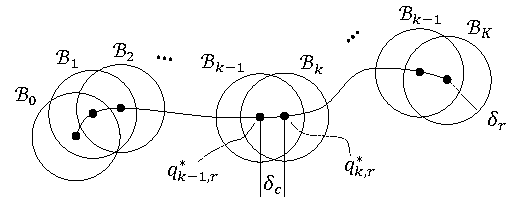
\includegraphics[width=0.7\columnwidth]{CoveringBallSequence}
    \caption{Example covering ball sequence for an example reference path with a distance along the path of $\ballseparation$ between each ball. Given that the path is $\deltar$-robust, each ball is a subset of $\robotCvalid$.}
    \label{fig:covering_ball_sequence}
\end{figure}


\subsection{Construction of a $\deltar$-similar Path}
\label{sec:delta_sim_traj_construction}

The objective here is to show with probability approaching $1$, the planner generates a $\deltar$-similar path to some robustly-feasible solution given enough time.  If an alternate path is found and the algorithm terminates before generating a $\deltar$-similar path then this is still sufficient for probabilistic completeness.  This analysis is similar to \cite{LiAOKP2016}, and is based on a covering ball sequence of the optimal  $\delta$-robust path $\refpathr$.

\begin{definition}[Covering Ball Sequence]
    \label{def:coveringballseq}
    Given a path $\rspacepath : [0, 1] \rightarrow \robotCvalid$, robust clearance $\deltar > 0$, a BestNearest distance $\bestneardist > 0$, and a distance value $0 < \ballseparation < \bestneardist < \deltar$; the covering ball sequence is defined as a set of $K + 1$ hyper-balls $\{ \hyperball_{\deltar}(\robotconfig_0), \dots, \hyperball_{\deltar}(\robotconfig_K) \}$ of radius $\deltar$, where $\robotconfig_k$ are defined such that:
    \begin{itemize}
        \item $\robotconfig_0 = \rspacepath(0)$;
        \item $\robotconfig_K = \rspacepath(1)$;
        \item $\textup{PathLength}(\robotconfig_{k-1}, \robotconfig_k) = \ballseparation$ for $k = 1, \dots, K$.
    \end{itemize}
\end{definition}
\noindent
Denote $\robotconfig^*_k$ to be the center of the $k^{th}$ covering hyper-ball for the reference path $\refpathr$. Fig.~\ref{fig:covering_ball_sequence} shows an example of a covering ball sequence.


The objective is to show that the vertex set of the planning tree after $n$ iterations $\rrtnodeset_n$ probabilistically contains a node within the goal set, i.e.
\begin{equation}
    \liminf_{n \rightarrow \infty} \pr( \rrtnodeset_n \cap \Pspacegoal \neq \emptyset ) = 1 \enspace .
\end{equation}
To do this, the analysis examines $K$ subsegments of the reference path $\refpathr$, based on the covering ball sequence for the reference path. If we can generate a robot path that is $\deltar$ similar to $\refpathr$, then given Assumption~\ref{ass:solvable_problem} and the properties of the reference path, the corresponding full space path will be a solution to the given planning problem.

Let $A_k^{(n)}$ be the event that on the $n^{th}$ iteration of the algorithm, it generates a $\deltar$-similar path to the $k^{th}$ subsegment of $\refpathr$.  This of course requires two events to occur: the node generated from the prior propagation covering segment $k-1$ must be selected for expansion, and the expansion must then produce a $\deltar$-similar path to the current segment.  Then, let $E_k^{(n)}$ be the event that for segment $k$, $A_k^{(n)}$ has occurred for some $i \in [1,n]$, i.e. $E_k^{(n)}$ indicates whether the algorithm has constructed the $\deltar$-similar edge for subsegment $k$. From these definitions, the goal then is to show that
\begin{equation}
    \lim_{n \rightarrow \infty} \pr(\textrm{Success}) = \lim_{n \rightarrow \infty} \pr\left( E^{(n)}_K \right) = 1 \enspace.
    \label{eqn:initial_pr_limit}
\end{equation}

We start by considering the probability of failing to generate an arbitrary segment $1 \leq k \leq K$. Then 
\begin{equation}
\begin{split}
    \pr&\left( \neg E^{(n)}_k \right) \\
       &= \pr\left( \neg A^{(1)}_k \cap \dots \cap \neg A^{(n)}_k \right) \\
       &= \pr\left( \neg A^{(1)}_k \right) \pr\left( \neg A^{(2)}_k \mid \neg A^{(1)}_k \right) \cdot \dots \\
       &\hspace{1.5cm} \cdot \pr\left( \neg A^{(n)}_k \mid \neg A^{(1)}_k \cap \dots \cap \neg A^{(n-1)}_k \right) \\
       &= \prod_{i=1}^n \pr\left( \neg A^{(i)}_k \mid \neg E^{(i-1)}_k \right) \enspace .
\end{split}
\label{eqn:fail_enk}
\end{equation}
Note the definition of $\neg E^{(i-1)}_k$ is what allows us to collapse the product into a concise form.


The probability that $\neg A^{(i)}_k$ happens given $\neg E^{(i-1)}_k$ is equivalent to the probability that we have not yet generated a $\deltar$-similar path for segment $k-1$ (i.e. $\pr( \neg E^{(i-1)}_{k-1} )$) plus the probability that the previous segment has been generated, but we fail to generate the current segment:
\begin{equation}
\begin{split}
    \pr&\left( \neg A^{(i)}_k \mid \neg E^{(i-1)}_k \right) \\
    &= \pr\left( \neg E^{(i-1)}_{k-1} \right) + \pr\left( E^{(i-1)}_{k-1} \right) \\
    &  \hspace{1.7cm} \cdot \pr\left( \neg A_k^{(i)} \mid E_{k-1}^{(i-1)} \cap \neg E_k^{(i-1)} \right), \\
\end{split}
\end{equation}
which we can rewrite in terms of $A_k^{(i)}$ instead of $\neg A_k^{(i)}$:
\begin{equation}
\begin{split}
    \pr&\left( \neg A^{(i)}_k \mid \neg E^{(i-1)}_k \right) \\
       &= \pr\left( \neg E^{(i-1)}_{k-1} \right) + \pr\left( E^{(i-1)}_{k-1} \right) \\
       &  \hspace{1.7cm} \cdot \left(1 - \pr\left( A_k^{(i)} \mid E_{k-1}^{(i-1)} \cap \neg E_k^{(i-1)} \right) \right) \enspace . \\
\end{split}
\end{equation}
Then multiplying out the last term we get
\begin{equation}
\begin{split}
    \pr&\left( \neg A^{(i)}_k \mid \neg E^{(i-1)}_k \right) \\
       &= \pr\left( \neg E^{(i-1)}_{k-1} \right) + \pr\left( E^{(i-1)}_{k-1} \right) \\
       &  \hspace{0.65cm} - \pr\left( E^{(i-1)}_{k-1} \right) \pr\left( A_k^{(i)} \mid E_{k-1}^{(i-1)} \cap \neg E_k^{(i-1)} \right) \enspace . \\
\end{split}
\end{equation}
Finally, summing the first two terms, we arrive at
\begin{equation}
\begin{split}
    \pr&\left( \neg A^{(i)}_k \mid \neg E^{(i-1)}_k \right) \\
       &= 1 - \pr\left( E^{(i-1)}_{k-1} \right) \pr\left( A_k^{(i)} \mid E_{k-1}^{(i-1)} \cap \neg E_k^{(i-1)} \right) \enspace .
\end{split}
\end{equation}
Two events need to happen in order to generate a path to the next hyperball; an appropriate node must be selected for expansion, and Connect$(\dots)$ must generate a $\deltar$-similar path segment, assuming that the appropriate node has already been selected. Denote the probability of these events at iteration $i$ as $\selectprobability$ and $\propagationprobability$ respectively. Then
\begin{equation}
    \pr\left( \neg A^{(i)}_k \mid \neg E^{(i-1)}_k \right) = 1 - \pr\left( E^{(i-1)}_{k-1} \right) \selectprobability \propagationprobability \enspace .
    \label{eqn:fail_aik}
\end{equation}

\noindent
As we are examining this probability in the limit, we will instead draw a bound on this probability to put it in a form we can easily examine the limit for. To do so, we must carefully consider the values of $\selectprobability$ and $\propagationprobability$.  In Section~\ref{sec:select}, it will be shown that $\selectprobability$ is a generally decreasing function, but converges to a finite value $\selectbound > 0$ in the limit.  Therefore we let $\selectbound$ be a lower bound of $\selectprobability$.  Then in Section~\ref{sec:prop}, $\propagationprobability$ will similarly be shown to be positive and lower-bounded; in particular $\selectprobability \propagationprobability \leq \selectbound$.  Taking $\selectbound$ as constant, we can bound Eq.~\eqref{eqn:fail_aik} as
\begin{equation}
    \pr\left( \neg A^{(i)}_k \mid \neg E^{(i-1)}_k \right) \leq 1 - \pr\left( E^{(i-1)}_{k-1} \right) \selectbound \enspace .
    \label{eqn:fail_aik_bound}
\end{equation}
Combining equations \eqref{eqn:fail_aik_bound} and \eqref{eqn:fail_enk} we have
\begin{equation}
    \pr\left( \neg E^{(n)}_k \right) \leq \prod_{i=1}^n \left(1 - \pr\left( E^{(i-1)}_{k-1} \right) \selectbound \right) \enspace .
\end{equation}
Denote $y^{(n)}_k = \prod_{i=1}^n \left(1 - \pr\left( E^{(i-1)}_{k-1} \right) \selectbound \right)$. Then
\begin{equation}
    \pr\left( \neg E^{(n)}_k \right) \leq y^{(n)}_k \enspace .
    \label{eqn:fail_enk_bound}
\end{equation}
We will show using induction over $k$, that Eq.~\eqref{eqn:fail_enk_bound} tends to 0 as $n \rightarrow \infty$, and thus $\lim_{n \rightarrow \infty} \pr(\textrm{Success}) = 1$\\

\noindent
\textbf{Base case $(k = 1)$:}\\
Note that $\pr(E^{(i)}_{0}) = 1$ because the start node always exists. Then 
\begin{equation}
\begin{split}
    \lim_{n \rightarrow \infty} \pr\left( \neg E^{(n)}_1 \right) 
        &\leq \lim_{n \rightarrow \infty} \prod_{i=1}^n \left(1 - \pr\left( E^{(i-1)}_{0} \right) \selectbound \right) \\
        &=    \lim_{n \rightarrow \infty} \prod_{i=1}^n \left(1 - \selectbound \right) \\
        &=\lim_{n \rightarrow \infty} \left(1 - \selectbound \right)^n = 0 \enspace .
\end{split}
\end{equation}

\noindent
\textbf{Induction hypothesis: }
\begin{equation}
    \lim_{n \rightarrow \infty} \pr\left( \neg E^{(n)}_m \right) = 0 \textrm{ for } m = 1, 2, \dots, k - 1 \enspace .
    \label{eqn:induction_hypothesis}
\end{equation}
Note that this implies $\lim_{n \rightarrow \infty} \pr( E^{(n)}_m ) = 1$ for $m = 1, 2, \dots, k - 1$.\\

\noindent
\textbf{Induction step ($2 \leq k \leq K$): }\\
Consider the log of the bound on $\pr\left( \neg E^{(n)}_k \right)$:
\begin{equation}
    \log y^{(n)}_k = \sum_{i=1}^n \log\left( 1 - \pr\left( E^{(i-1)}_{k-1} \right) \selectbound \right) \enspace .
    \label{eqn:logy}
\end{equation}
Denote $x = \pr\left( E^{(i-1)}_{k-1} \right) \selectbound$. Given that $0 \leq x < 1$, and writing the Taylor series expansion of $\log\left( 1 - x \right)$ centered at $x = 0$ we have
\begin{equation}
    \log \left( 1 - x \right) = - \sum_{m=1}^\infty \frac{x^m}{m} \enspace .
    \label{eqn:log1minusx}
\end{equation}
Substituting Eq.~\eqref{eqn:log1minusx} back into Eq.~\eqref{eqn:logy} we get
\begin{equation}
    \log y^{(n)}_k = - \sum_{i=1}^n \sum_{m=1}^\infty \frac{\left( \pr\left( E^{(i-1)}_{k-1} \right) \selectbound \right)^m}{m} \enspace .
\end{equation}
Dropping all but the first term in the infinite sum we get the bound
\begin{equation}
    \log y^{(n)}_k \leq -\sum_{i=1}^n \pr\left( E^{(i-1)}_{k-1} \right) \selectbound \enspace .
\end{equation}
Rearranging terms yields
\begin{equation}
    \log y^{(n)}_k \leq -\selectbound \sum_{i=1}^n \pr\left( E^{(i-1)}_{k-1} \right) \enspace .
\end{equation}
We now use the induction hypothesis. We know that $\pr( E^{(n)}_{k-1} ) \rightarrow 1$ as $n \rightarrow \infty$, thus $\sum_{i=1}^n \pr( E^{(i-1)}_{k-1} ) \rightarrow \infty$. Then
\begin{equation}
    \lim_{n \rightarrow \infty} \log y^{(n)}_k \leq -\selectbound \sum_{i=1}^n \lim_{n \rightarrow \infty} \pr\left( E^{(i-1)}_{k-1} \right) = -\infty \enspace .
    \label{eqn:logy_bound}
\end{equation}
Taking the log of Eq.~\eqref{eqn:fail_enk_bound} and combining with Eq.~\eqref{eqn:logy_bound} we get
\begin{equation}
    \lim_{n \rightarrow \infty} \log \pr\left( \neg E^{(n)}_k \right) \leq \lim_{n \rightarrow \infty} \log y^{(n)}_k = -\infty
\end{equation}
and therefore
\begin{equation}
    \lim_{n \rightarrow \infty} \pr\left( \neg E^{(n)}_k \right) = 0 ,
\end{equation}
which completes the induction step.


Thus, given that $\pr(\neg E^{(n)}_k) \rightarrow 0$ as $n \rightarrow \infty$ for any $1 \leq k \leq K$
\begin{equation}
    \lim_{n \rightarrow \infty} \pr(\textrm{Success}) = \lim_{n \rightarrow \infty} \left( 1 - \pr\left( \neg E^{(n)}_K \right) \right) = 1 \enspace.
\end{equation}



%%%%%%%%%%%%%%%%%%%%%%%%%%%%%%%%%%%%%%%%%%%%%%%%%%%%%%%%%%%%%%%%%
%% Node Selection
\subsubsection{Selection of an appropriate node ($\selectbound$):}
\label{sec:select}

% \begin{figure}
%     \centering
%     
\includegraphics{placeholder}
%     \caption{Figure for Sec.~\ref{sec:select} and Sec.~\ref{sec:prop}}
%     \label{fig:select_and_prop}
% \end{figure}
First, we define the following restriction on the definition of $\bestneardist$: 

\begin{definition}[$\bestneardist$ Restriction]
\label{prop:bestnear_requirement}
    For a reference path $\refpathr$ with robustness $\deltar$, $\bestneardist$ is defined such that $\innerballsize = \deltar - \bestneardist > 0$.
\end{definition}

The proof that $\selectbound > 0$ follows directly from the related work of \cite{LiAOKP2016} (proof of Lemma 23).  To summarize, due to best-nearest neighbors selection, there exists a positive-measure region around the minimum cost vertex $\pstatenear$ which observes the optimal reference path in which its cost dominates all other nearby nodes, and therefore, when $\pstaterand$ is drawn in this volume, $\pstatenear = (\pstatenearfull)$ is guaranteed to be selected (Fig.~\ref{fig:Yanbo_lemma_23_figure}).  Since our approach follows an equivalent sampling and nearest neighbor method to \cite{LiAOKP2016} (as shown in Sec.~\ref{sec:nn_equiv}), 
\begin{equation}
    \selectbound = \frac{\mu\left( \hyperball_{\innerballsize}\big( \pstate_k^* \big) \cap \hyperball_{\bestneardist}\big( \pstatenear \big) \right)}{\mu\left( \pspace \right)} > 0
\end{equation}
follows directly.

\begin{figure}[t]
    \centering
    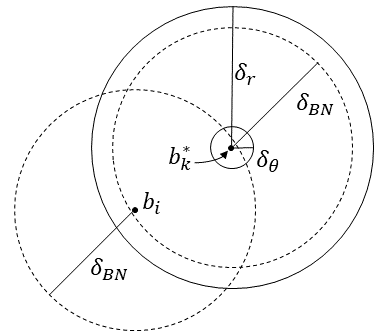
\includegraphics[width=0.3\columnwidth]{nearest_neighbour_domination_region}
    \caption{Minimum domination region for a node $\pstate_i$, adapted from \cite{LiAOKP2016} Lemma 23. Sampling $\pstaterand$ in the shaded region guarantees that a node $\pstatenear \in \hyperball_{\deltar}(\pstate_k^*)$ is selected for propagation so that either $\pstatenear = \pstate_i$ or $\cost(\pstatenear) < \cost(\pstate_i)$.}
    \label{fig:Yanbo_lemma_23_figure}
\end{figure}

To show that $\selectbound < 1$, we need only consider the case when there are at least 2 nodes in $\rrtnodeset$.

%%%%%%%%%%%%%%%%%%%%%%%%%%%%%%%%%%%%%%%%%%%%%%%%%%%%%%%%%%%%%%%%%
%% Node Propagation
%%%%%%%%%%%%%%%%%%%%%%%%%%%%%%%%%%%%%%%%%%%%%%%%%%%%%%%%%%%%%%%%%
\subsubsection{$\deltar$-similar Propagation ($\propagationprobability$):}
\label{sec:prop}
Given that our nearest neighbor method is non-standard, and operating in the full configuration space $\pspace$, we need to carefully consider how this affects the propagation probability $\propagationprobability$. Given the kinematic model of our robot system, it is straightforward to show that the system in robot space is Small-Time Locally Controllable (STLC), i.e. $\robotconfig$ can be instantaneously moved in any direction, barring the presence of obstacles or configuration space limits.  

Then, based on the construction of the covering ball sequence and the $\bestneardist$ restriction, the following lemma holds.

\begin{lemma}
    \label{lem:rand_to_next_dist}
    If $\pstaterand$ is within the minimum domination region as described in \cite{LiAOKP2016} Lemma 23 (Fig.~\ref{fig:Yanbo_lemma_23_figure}), then $\robotconfigrand \in \hyperball_{\deltar}(\robotconfig^*_k)$ and Connect() will generate a segment that is $\deltar$-similar to segment $k$ of the reference path.
\end{lemma}



\noindent
{\bf Proof.}
Assume that $\pstaterand \in \hyperball_{\innerballsize}(\pstate^*_{k-1})$. Then we have
\begin{align*}
    d_\robotconfig(\robotconfigrand, \robotconfig^*_k)  &\leq d_\pstate(\pstaterand, \pstate^*_k) \\
                                                        &\leq d_\pstate(\pstaterand, \pstate^*_{k-1}) + d_\pstate(\pstate^*_{k-1}, \pstate^*_k) \\
                                                        &\leq \innerballsize + \ballseparation = \deltar - \bestneardist + \ballseparation \enspace.
\end{align*}
Then by construction of the covering ball sequence, we have that $\ballseparation -\bestneardist < 0$ and thus $d_\robotconfig(\robotconfigrand, \robotconfig^*_k) < \deltar$. In addition, we have that the straight line between $\robotconfignear$ as selected by $\robotconfigrand$ is entirely contained in $\hyperball_{\deltar}(\robotconfig^*_{k-1})$, and thus is also in $\robotCvalid$ as the reference path is optimal $\delta$-robust. We then have that the path generated by Connect is $\deltar$-similar to the $k^{th}$ segment of the reference path.
\qed

\begin{lemma}
    The probability of covering segment $k$ at iteration $i$, given that we have not yet covered segment $k$ but we have covered segment $k-1$
    $$\pr\left( A_k^{(i)} \mid E_{k-1}^{(i-1)} \cap \neg E_k^{(i-1)} \right) = \selectprobability \propagationprobability$$
    is lower-bounded by $\selectbound$.
\end{lemma}

\noindent
{\bf Proof.}
Consider two possible events. First, that $\pstaterand$ is within the minimum domination region (Fig.~\ref{fig:Yanbo_lemma_23_figure}) of $\Pstatenear$. If $\pstaterand$ is within the minimum domination region of $\Pstatenear$, then by Lemma~\ref{lem:rand_to_next_dist}, Connect() will generate a $\deltar$-similar segment with probability 1. Denote this event as $B$. Second, the event that $\pstaterand$ is somewhere else. Denote this event as $C$. Then we can bound $\pr( A_k^{(i)} \mid E_{k-1}^{(i-1)} \cap \neg E_k^{(i-1)})$ by considering only $B$:
\begin{align*}
    \pr\left( A_k^{(i)} \mid E_{k-1}^{(i-1)} \cap \neg E_k^{(i-1)} \right) 
        &= \pr(B) + \pr(C) \\
        &\geq \pr(B) \geq \selectbound \enspace .
\end{align*}
\qed
